\section{Métodos supervisados}
\begin{frame}{Métodos supervisados}
\begin{columns}
\begin{column}{0.9\textwidth}
\begin{defi}
Son aquellos que buscan inferir una relación estocástica entre dos grupos de variables, predictoras a partir de un conjunto de datos procedentes de observaciones simultáneas de ambos conjuntos. 
\end{defi}

Si se estudian varias variables de manera simultánea, se dividen en los siguientes tipos:
\begin{itemize}
\item Variables predictoras, son las variables independientes, se denotarán por el vector aleatorio $\mathbf{x}=[X_1,\ldots, X_p]$ 
\item Variables respuesta, son las variables dependientes, se denotarán como el vector aleatorio $\mathbf{y}=[Y_1,\ldots, Y_K]$ y como $Y$ cuando $K=1$.
\end{itemize}
\end{column}
\end{columns}
\end{frame}

\begin{frame}{Métodos supervisados}
\begin{columns}
\begin{column}{0.9\textwidth}
Se trabajará con muestras aleatorias simples de $N$ observaciones de las $K+p$ variables, obteniéndose las siguientes matrices:
\begin{defi}
Se llama matriz de datos $\mathbf{X}$ a la matriz de tamaño $N\times p$ cuyas filas $\mathbf{x}_i,\enspace i=1,\ldots,N$ representan una observación de las $p$ variables predictoras.
\end{defi}
\begin{defi}
Se llama matriz de respuestas $\mathbf{Y}$ a la matriz de tamaño $N\times K$ cuyas filas $\mathbf{y}_i,\enspace i=1,\ldots,N$ representan una observación de las $K$ variables respuesta.
\end{defi}
\end{column}
\end{columns}
\end{frame}

\begin{frame}{Métodos supervisados}
\begin{columns}
\begin{column}{0.9\textwidth}
Por tanto, se recogen $N$ observaciones $(\mathbf{x}_i,\mathbf{y}_i)$ obteniéndose un vector de longitud $K+p$.

Los métodos supervisados buscan estimar una relación estocástica que se llamará predictor que conocido el valor de las variables predictoras $\mathbf{x}_0$, se pueda hacer una predicción del valor de las variables respuesta $\mathbf{y}_0$, que se denota por $\mathbf{\hat{y}}_0$.
\end{column}
\end{columns}
\end{frame}

\subsection{Métodos lineales para regresión}
\begin{frame}{Métodos supervisados}
\begin{columns}
\begin{column}{0.9\textwidth}
El objetivo de la regresión lineal es estudiar como un conjunto de variables respuesta están relacionadas con una combinación lineal de las variables predictoras. 
\end{column}
\end{columns}
\end{frame}

\begin{frame}{Métodos supervisados}
\begin{columns}
\begin{column}{0.9\textwidth}
Tomamos el modelo en el que: 
\begin{equation}
Y=f(\mathbf{x})+\varepsilon
\end{equation}
donde $\varepsilon$ cumple:
\begin{itemize}
\item $\mathbb{E}(\varepsilon)=0$
\item $Var(\varepsilon)=\sigma^2$
\end{itemize}
A mayores se puede asumir que $\varepsilon\sim N(0,\sigma^2)$
\end{column}
\end{columns}
\end{frame}

\begin{frame}{Métodos supervisados}
\begin{columns}
\begin{column}{0.9\textwidth}
En la regresión lineal se asume que $f$ es de la siguiente manera:
\begin{equation}
f(\mathbf{x})=\beta_0+\sum_{j=1}^p \beta_j X_j
\end{equation}
\begin{itemize}
\item $\beta=[\beta_0,\beta_1,\ldots,\beta_p]^T$ es el vector con los parámetros de regresión.
\item Añadiendo a $\mathbf{x}$ la variable $X_0=1$ se puede expresar f: 
\end{itemize}

\begin{equation}
f(\mathbf{x})=\mathbf{x}\beta
\end{equation}

Tomando $N$ observaciones, se puede obtener el vector $\mathbf{\hat{y}}$:
\begin{equation}\label{eq: predicción}
\mathbf{\hat{y}}=\mathbf{X}\beta
\end{equation}

\end{column}
\end{columns}
\end{frame}


\begin{frame}{Métodos supervisados}
\begin{columns}
\begin{column}{0.9\textwidth}
Se pueden estimar los parámetros de regresión mediante el método de los mínimos cuadrados:
\begin{equation}
\hat{\beta}=(\mathbf{X}^T\mathbf{X})^{-1}\mathbf{X}^T \mathbf{y}
\end{equation}

Sustituyendo en la ecuación \ref{eq: predicción}
\begin{equation}
\mathbf{\hat{y}}= \mathbf{X}(\mathbf{X}^T\mathbf{X})^{-1}\mathbf{X}^T \mathbf{y}
\end{equation}

\end{column}
\end{columns}
\end{frame}




\begin{frame}{Métodos supervisados}
\begin{columns}
\begin{column}{0.9\textwidth}

Supóngase lo siguiente: 
\begin{itemize}
\item $\mathbf{x}\sim N(\mu,\Sigma)$ del que obtenemos la matriz de datos $\mathbf{X}$ de tamaño $N\times p$. 
\item $\mathbf{y}=\mathbf{X}\beta+\varepsilon$ donde $\varepsilon\sim N(0,\sigma^2\mathbf{I}_N)$.
\end{itemize}
\end{column}
\end{columns}
\end{frame}



\begin{frame}{Métodos supervisados}
\begin{columns}
\begin{column}{0.9\textwidth}
Se cumplen las siguientes propiedades: 
\begin{itemize}
\item El vector $\mathbf{y}\sim N(\mathbf{X}\beta,\sigma^2\mathbf{I}_N)$
\item El vector $\hat{\beta}$ es un estimador insesgado.
\item La varianza de $Var(\hat{\beta})=\sigma^2(\mathbf{X}^T\mathbf{X})^{-1}$.
\item El estimador $\displaystyle\hat{\sigma}^2=\dfrac{1}{N-p-1}\sum_{i=1}^N(y_i-\hat{y}_i)^2$ es un estimador insesgado de $\sigma^2$ y además $\displaystyle\hat{\sigma}^2\sim \dfrac{\sigma^2}{N-p-1}\chi_{N-p-1}^2$
\end{itemize}

\end{column}
\end{columns}
\end{frame}

\begin{frame}{Métodos supervisados}
\begin{columns}
\begin{column}{0.9\textwidth}
Se puede definir un estadígrafo de contraste para comprobar si un conjunto de variables es estadísticamente significativo en el modelo. 
\begin{equation}\label{eq: Estimador F}
F=\dfrac{\dfrac{(RSS_0-RSS_1)}{p_1-p_0}}{\dfrac{RSS_1}{N-p_1-1}}\sim F_{(p_1,p_0),(N-p_1-1)}
\end{equation}
\end{column}
\end{columns}
\end{frame}


\begin{frame}{Métodos supervisados}
\begin{columns}
\begin{column}{0.9\textwidth}
En el caso de que tengamos $K$ variables respuesta $Y_1,\ldots, Y_K$ entonces el modelo es:
\begin{equation}
Y_k=\beta_{0k}+\sum_{j=1}^p X_j\beta_{jk}+\varepsilon_k = f_k(\textbf{x})+\varepsilon_k, \quad k=1,\ldots K
\end{equation}
donde $\varepsilon_k \sim N(0,\sigma_k^2)\enspace\forall k=1,\ldots,K$ que pueden o no estar correlacionados. Al tomar $N$ observaciones se puede expresar de manera matricial
\begin{equation}
\mathbf{Y=XB+E}
\end{equation}
donde $\mathbf{E}$ es la matriz $N\times K$ de errores cometidos en cada una de las observaciones.
\end{column}
\end{columns}
\end{frame}

\begin{frame}{Métodos supervisados}
\begin{columns}
\begin{column}{0.9\textwidth}
El método de los mínimos cuadrados, cambia en el caso de que los errores tengan matriz de covarianzas $\mathbf{\Sigma}$ conocida el $RSS$ se define de la siguiente manera: 
\begin{equation}
RSS(\textbf{B},\mathbf{\Sigma})=\sum_{i=1}^N(\mathbf{y}_i-f(\textbf{x}_i)) \mathbf{\Sigma}^{-1} (\mathbf{y}_i-f(\textbf{x}_i))^T
\end{equation}

donde $d(\mathbf{x}_i,\mathbf{x}_j)=\sqrt{(\mathbf{x}_i-\mathbf{x}_j) \mathbf{\Sigma}^{-1} (\mathbf{x}_i-\mathbf{x}_j)^T}$ es la distancia de Mahalanobis entre dos observaciones. 
\end{column}
\end{columns}
\end{frame}


\begin{frame}{Métodos supervisados}
\begin{columns}
\begin{column}{0.9\textwidth}
Se puede utilizar el estadígrafo $F$ de la ecuación \ref{eq: Estimador F} para seleccionar las variables del modelo. 

También se puede definir lo siguiente: 
\begin{defi} 
Llamamos errores cuadrados acumulados penalizados, \emph{PRSS}, a la suma de los cuadrados de los errores cometidos con el modelo lineal que usa el  vector de parámetros $\beta$, añadiendo un término regulador $\lambda >0$: 
\begin{equation}
PRSS(\beta)=\sum_{i=1}^n(\textbf{y}_i-\textbf{x}_i\beta)^2+\lambda\sum_{j=1}^p\beta_j^2
\end{equation}
\end{defi}
Esto permite dar una forma de regular los tamaños de los parámetros $\beta$
\end{column}
\end{columns}
\end{frame}

\subsection{Clasificación}
\begin{frame}{Métodos supervisados}
\begin{columns}
\begin{column}{0.9\textwidth}
La clasificación es el caso donde la variable respuesta es cualitativa. 
Hay dos tareas a realizar:
\begin{itemize}
 \item Discriminación: Estudiar las características que diferencian a cada una de las poblaciones. 
 \item Clasificación: Asignar nuevas observaciones a una de las poblaciones 
\end{itemize}
\end{column}
\end{columns}
\end{frame}


\begin{frame}{Métodos supervisados}
\begin{columns}
\begin{column}{0.9\textwidth}
Si tenemos dos poblaciones $\pi_1, \pi_2$ de las cuales se conocen las funciones de probabilidad de cada una de ellas $f_1,f_2$ , entonces si se conoce la probabilidad de de clasificación de clasificar en la población incorrecta, $P(1|2), P(2|1)$, entonces: 
\begin{equation}
\begin{split}
P(i|\textbf{x}_0)&=\dfrac{P(\textbf{x}_0|i)P(i)}{P(1)P(\textbf{x}_0|1)+P(2)P(\textbf{x}_0|2)}\\&=\dfrac{f_i(\mathbf{x}_0)P(i)}{P(1)f_1(\mathbf{x}_0)+P(2)f_2(\mathbf{x}_0)}
\end{split}
\end{equation}
donde $i=1,2$
\end{column}
\end{columns}
\end{frame}

\begin{frame}{Métodos supervisados}
\begin{columns}
\begin{column}{0.9\textwidth}
Se utilizará el concepto de función discriminante: 
\begin{defi}
Se llama función discriminante, $f_{d}$ aquella que:
\begin{equation}
f_{d}:\mathbf{\Omega}\longrightarrow \mathbb{R},
\end{equation}
donde $\mathbf{\Omega}$ es el espacio de observaciones posibles, definida de tal manera que si $f_{d}(\textbf{x}_0)>0\Rightarrow \textbf{x}_0\in \pi_i$ y en caso contrario $\textbf{x}_0\notin \pi_i$. 
\end{defi}
\end{column}
\end{columns}
\end{frame}

\begin{frame}{Métodos supervisados}
\begin{columns}
\begin{column}{0.9\textwidth}
Teniendo esta definición en mente para dos poblaciones y teniendo  en cuenta el coste de clasificación errónea, se obtiene la siguiente función discriminante:

\begin{equation}
f_d(\mathbf{x}_0)=\dfrac{f_1(\textbf{x}_0)P(1)}{c(1|2)}-\dfrac{f_2(\textbf{x}_0)P(2)}{c(2|1)}
\end{equation}

Si se sustituye $f_1,f_2$ por funciones normales se obtiene la función discriminante: 
\begin{equation}
\begin{split}
f_d(\mathbf{x})&=(\textbf{x}-\mu_1)^T \mathbf{\Sigma}^{-1}(\textbf{x}-\mu_1)+log\left(\dfrac{P(1)}{c(1|2)}\right)\\&-(\textbf{x}-\mu_2)^T \mathbf{\Sigma}^{-1} (\textbf{x}-\mu_2)-log\left(\dfrac{P(2)}{c(2|1)}\right)
\end{split}
\end{equation}

\end{column}
\end{columns}
\end{frame}

\begin{frame}{Métodos supervisados}
\begin{columns}
\begin{column}{0.9\textwidth}

El análisis canónico de poblaciones busca identificar las direcciones de mayor diferenciación entre las distintas $L$ poblaciones.
\begin{defi}
\noindent La covarianza intragrupo de un par de variables en la $l$-ésima población:
\begin{equation}
W_l(X_j,X_{j'})=\dfrac{1}{N_l}\sum_{i\in I_l} (x_{ij}-\overline{x}_{jl})(x_{ij'}-\overline{x}_{j'l})
\end{equation}   
\end{defi}
\begin{defi}
La covarianza intergrupos
\begin{equation}
B(X_j,X_{j'})=\sum_{l=1}^L\dfrac{N_l}{N}(\overline{x}_{jl}-\overline{x}_{j})(\overline{x}_{j'l}-\overline{x}_{j'})
\end{equation}   
\end{defi}

\end{column}
\end{columns}
\end{frame}

\begin{frame}{Métodos supervisados}
\begin{columns}
\begin{column}{0.9\textwidth}

Entonces se buscan combinaciones lineales que maximicen la varianza entre grupos respecto la varianza por tanto, se busca maximizar la función
\begin{equation}
f(\mathbf{a})=\dfrac{\mathbf{a}^T\mathbf{Ba}}{\mathbf{a}^T\mathbf{Ta}}
\end{equation}

Tomando la restricción $\mathbf{a}^T\mathbf{T}\mathbf{a}$ y aplicando los multiplicadores de Lagrange, se obtiene que el vector $\mathbf{a}$ es el vector propio con valor propio máximo $\lambda$ de la matriz $\mathbf{T}^{-1}\mathbf{B}$.

\end{column}
\end{columns}
\end{frame}

\input{Documentos Extra/Redes  neuronales.tex}

\subsection{Árboles de decisión y bosques aleatorios.}
\begin{frame}{Métodos supervisados}
\begin{columns}
\begin{column}{0.9\textwidth}
\begin{defi}
Los árboles de decisión son conjuntos de reglas discriminantes que fraccionan el espacio de observaciones en regiones donde se modeliza la variable respuesta de manera sencilla. En el proceso de ajuste generan un grafo de tipo árbol con un nodo raíz y los nodos hoja representan cada una de las regiones resultantes. 
\end{defi}
\end{column}
\end{columns}
\end{frame}

\begin{frame}{Métodos supervisados}
\begin{columns}
\begin{column}{0.9\textwidth}
Conceptos importantes:
\begin{itemize}
\item Partición de indices $(j,s)$.
\item Nodo terminal o nodo hoja.
\item Nodo padre y nodo hijo.
\item Profundidad y tamaño del árbol.
\end{itemize}
\begin{center}
\begin{figure}[ht]
  \subfloat[División de $\mathbb{R}^p$]{
   \label{f:división}
    \includegraphics[width=0.25\textwidth]{Documentos Extra/Imagenes/Regiones árboles.png}}
  \subfloat[Diagrama resultante]{
   \label{f:diagrama arbol}
    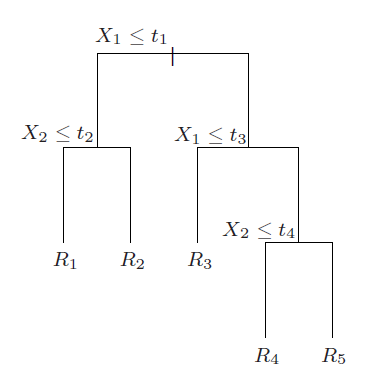
\includegraphics[width=0.25\textwidth]{Documentos Extra/Imagenes/Diagrama de arbol.png}}
 \caption{Representación de la división de $\mathbb{R}^p$ y el diagrama de árbol \\resultante.}
 \label{f:MARC1}
\end{figure}
\end{center}
\end{column}
\end{columns}
\end{frame}
\subsubsection{Árboles de regresión}
\begin{frame}{Métodos supervisados}
\begin{columns}
\begin{column}{0.9\textwidth}
\textbf{Árboles de regresión}

Sea el caso en el que la variable respuesta es cuantitiva y las variables predictoras son cuantitativas o cualitativas.

Tras haber ajustado el árbol hasta tener un tamaño $|T|=M$ resultando en las regiones $R_1,\ldots, R_M$. Entonces el predictor será el siguiente: 
\begin{equation}
\hat{f}(\mathbf{x})=\sum_{m=1}^M \hat{f}_m(\mathbf{x})\cdot \mathbf{1}_m(\mathbf{x})
\end{equation}
donde $\mathbf{1}_m(\mathbf{x})$ es la función característica de la región $R_m,\enspace \forall m=1,\ldots, M$.
\end{column}
\end{columns}
\end{frame}

\begin{frame}{Métodos supervisados}
\begin{columns}
\begin{column}{0.9\textwidth}
\textbf{Árboles de regresión}

Si en cada región queremos que $\hat{f}_m$ sea una constante, $\hat{c}_m$. Utilizando el método de los mínimos cuadrados teniendo en cuenta la restricción de que sea constante se obtiene que: 
\begin{equation}
\hat{c}_m=\dfrac{1}{N_m}\sum_{i/\mathbf{x}_i\in R_m} y_i
\end{equation}
donde $N_m$ es la cantidad de observaciones que hay en la región $R_m \enspace \forall m=1,\ldots M$
\end{column}
\end{columns}
\end{frame}

\begin{frame}{Métodos supervisados}
\begin{columns}
\begin{column}{0.9\textwidth}
\textbf{Árboles de Regresión}

Una partición $(j,s)$ que particione el espacio en las dos regiones $R_{m_1},R_{m_2}$ es elegida si minimiza la siguiente cantidad:
\begin{equation}
\sum_{i/\mathbf{x}_i\in R_{m_1} } (y_i-\hat{c}_{m_1})^2+\sum_{i/\mathbf{x}_i\in R_{m_2} } (y_i-\hat{c}_{m_2})^2
\end{equation}

\end{column}
\end{columns}
\end{frame}

